\documentclass[10pt,a4paper]{article}
\usepackage[margin=2.1cm]{geometry}
\usepackage[T1]{fontenc}
\usepackage{lmodern,booktabs,graphicx,amsmath,xcolor,tabularx,float}
\usepackage[colorlinks=true,linkcolor=black,urlcolor=blue!60!black,citecolor=black]{hyperref}
\graphicspath{{../images/}}
\setlength{\parskip}{3pt}
\renewcommand{\arraystretch}{1.12}
\newcommand{\notecaption}[1]{\par\smallskip{\small #1}\par}
\title{\vspace{-1.2cm}\textbf{Does a forecast-driven Black--Litterman overlay add value to large-cap momentum?}\\[2pt]
\large Evidence from the point-in-time S\&P 500, 2003--2023}
\author{AimanxxAnsari\\\small\url{https://github.com/AimanxxAnsari/momentum-trading-strategy}}
\date{Research note}
\begin{document}
\maketitle
\vspace{-0.6cm}
\begin{abstract}
\noindent A long-only strategy selects the 25 strongest 12--1 month momentum stocks among the 50 largest S\&P 500
members, turns ARIMA return forecasts into Black--Litterman views and holds a max-Sharpe portfolio, rebalanced
quarterly with transaction costs. Over 2010--2023 it returned 12.2\% a year against 11.1\% for an
S\&P 500 proxy, but the gap is risk and factor exposure, not skill. Signal research finds no momentum premium in the
S\&P 500 over 2003--2023; the one signal with predictive power in the top 50 (each stock's historical mean return)
comes from the 2017--2023 growth rally. Fixing the portfolio construction with Grinold alphas, a factor risk model
and a benchmark-relative optimiser cuts turnover from 453\% to 28\% a year and leaves the strategy earning
about its benchmark. With the actual T-bill rate the strategy's Sharpe ratio is 0.625 against 0.640.
Relative to the index it is a momentum-and-growth tilt; across all 47 variants tested, factor alpha t-statistics
range from $-$1.79 to +1.02, and the best variant's deflated Sharpe ratio is 0.65--0.85,
short of the usual 0.95.
\end{abstract}

\section{Data and design}
\textbf{Data.} Daily Bloomberg prices, market capitalisations and book values for every company that was in the
S\&P 500 at any point in 2000--2023, and 168 quarterly constituent snapshots. The universe on each date is the 50
largest members of the most recent snapshot, so there is no survivorship bias. Three properties of the data shape
the analysis: prices are split-adjusted but there are no dividends (all returns are price returns); the earnings
field is empty, so value is measured by book-to-price only; and book value is stamped at the fiscal period end,
before publication, so it is lagged three months. Fama--French factors and the 1-month T-bill rate come from Kenneth
French's data library. The T-bill averaged 0.84\% a year over 2010--2023, against the constant 3\% assumed in
Phases~1--7.

\textbf{Design.} Every decision uses only data available on the rebalance date (the last trading day of each
quarter); holdings drift between rebalances; every portfolio, benchmarks included, pays 10\,bps per unit traded.
The analysis was built up in eight phases, each reported in its own notebook; the code is a tested Python package
(37 unit tests on synthetic data). All 47 variants of the strategy that were run are kept and corrected for in
Section~\ref{sec:inference}.

\section{The baseline strategy}
Black--Litterman combines a market-capitalisation prior $\pi = \delta\Sigma w_{\text{mkt}}$ with one absolute view per
stock (the ARIMA forecast minus the risk-free rate) and He--Litterman uncertainty $\Omega = \operatorname{diag}(\tau\Sigma)$,
with a Ledoit--Wolf covariance. The optimiser maximises the posterior Sharpe ratio, long-only, at most 20\% per stock.

\begin{table}[H]\centering\small
\notecaption{\textbf{Table 1.} Baseline, 2010--2023, walk-forward, after costs, price returns.}
\begin{tabular}{lrrrrrr}\toprule
& CAGR & Volatility & Sharpe (3\%) & Sharpe (T-bill) & Max drawdown & Turnover / yr\\\midrule
Strategy (baseline) & 12.2\% & 20.4\% & 0.52 & 0.63 & $-$33.0\% & 453\% \\
Cap-weighted top 50 & 11.5\% & 17.9\% & 0.53 & 0.65 & $-$30.0\% & 22\% \\
Cap-weighted S\&P 500 proxy & 11.1\% & 17.5\% & 0.52 & 0.64 & $-$33.6\% & 8\% \\
\bottomrule\end{tabular}
\end{table}
\vspace{-0.3cm}
The strategy's information ratio against the S\&P 500 proxy is 0.15 (t = 0.58). Adding the layers one at a time
shows that momentum selection, the optimiser and the ARIMA views each move the Sharpe ratio by 0.03 or less, while
turnover rises about sevenfold. Two diagnostics explain why: 63\% of the fitted ARIMA models are (0,0,0), so the
``forecasts'' are mostly each stock's historical mean return; and the optimiser concentrates the portfolio into a
median of 7 names at the 20\% cap.

\begin{figure}[H]\centering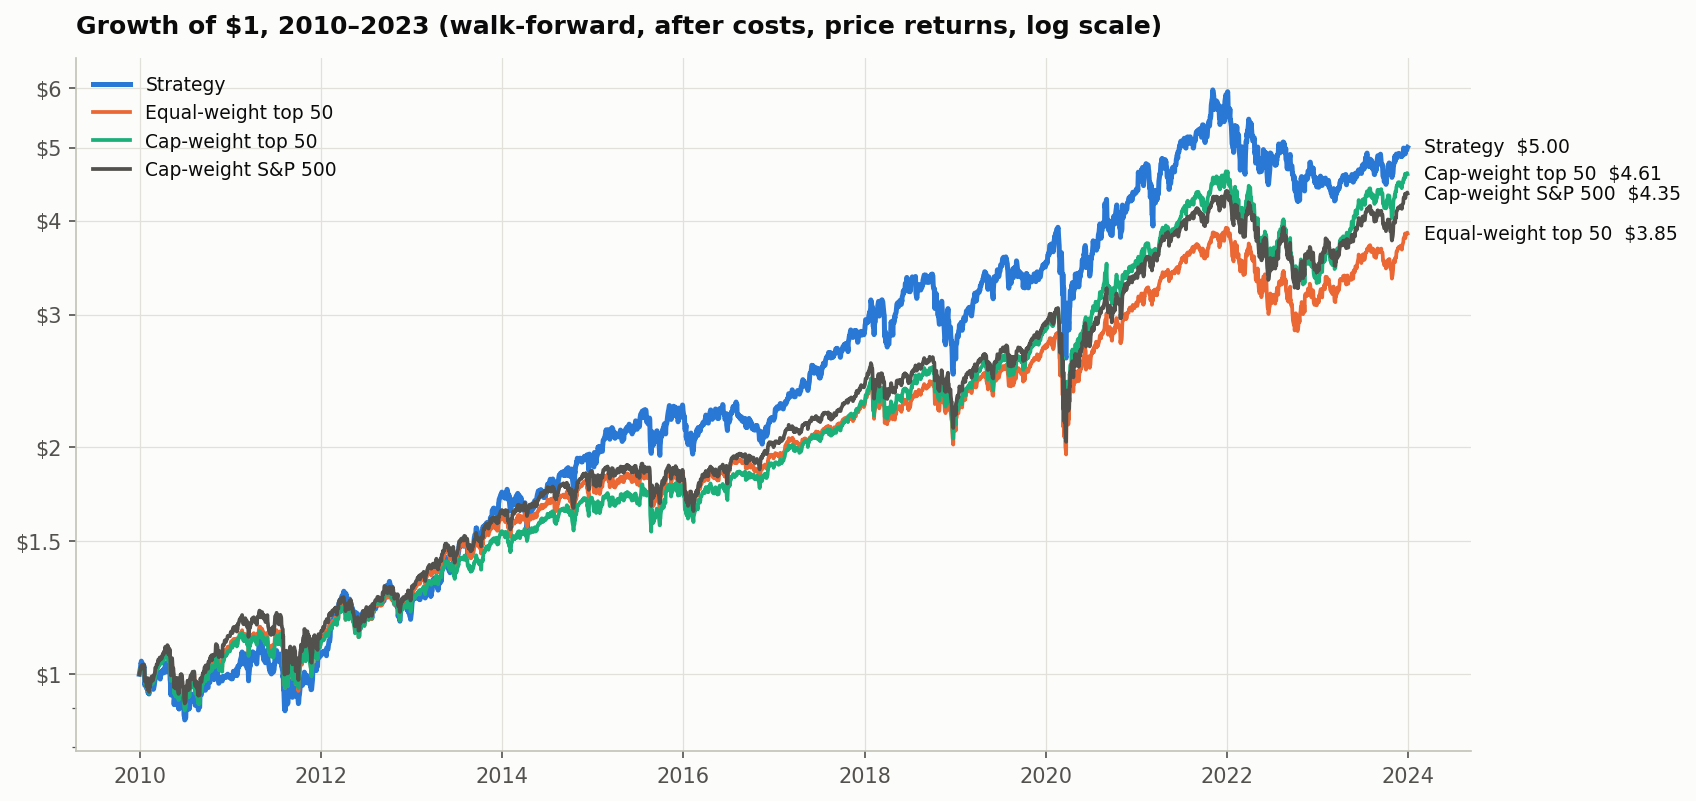
\includegraphics[width=0.66\textwidth]{equity_curve.png}
\notecaption{\textbf{Figure 1.} Growth of \$1, 2010--2023, after costs (from \texttt{main.ipynb}).}\end{figure}

\section{Is there a premium to capture?}
Eight signals were tested on their own, monthly over 2003--2023, for the whole point-in-time S\&P 500 and its 50
largest members: rank information coefficients (IC) at 1--12 month horizons with Newey--West t-statistics, three
sub-periods, quintile portfolios and Fama--MacBeth regressions.
\begin{itemize}\setlength\itemsep{1pt}
\item \textbf{No momentum premium.} For 12--1 momentum in the S\&P 500 the 3-month IC is $-$0.001 (t = $-$0.06) and
the top-minus-bottom quintile earned $-$1.8\% a year (t = $-$0.41). No signal is significant in the full index.
\item \textbf{The historical-mean signal is the growth rally.} It is the only significant signal in the top 50 (3-month
IC 0.056, t = 2.5), but its IC is +0.001, +0.034 and +0.136 in 2003--09, 2010--16 and 2017--23; with the other
signals as controls its Fama--MacBeth t-statistic is 1.21. It is correlated $-0.35$ with book-to-price.
\end{itemize}

\begin{figure}[H]\centering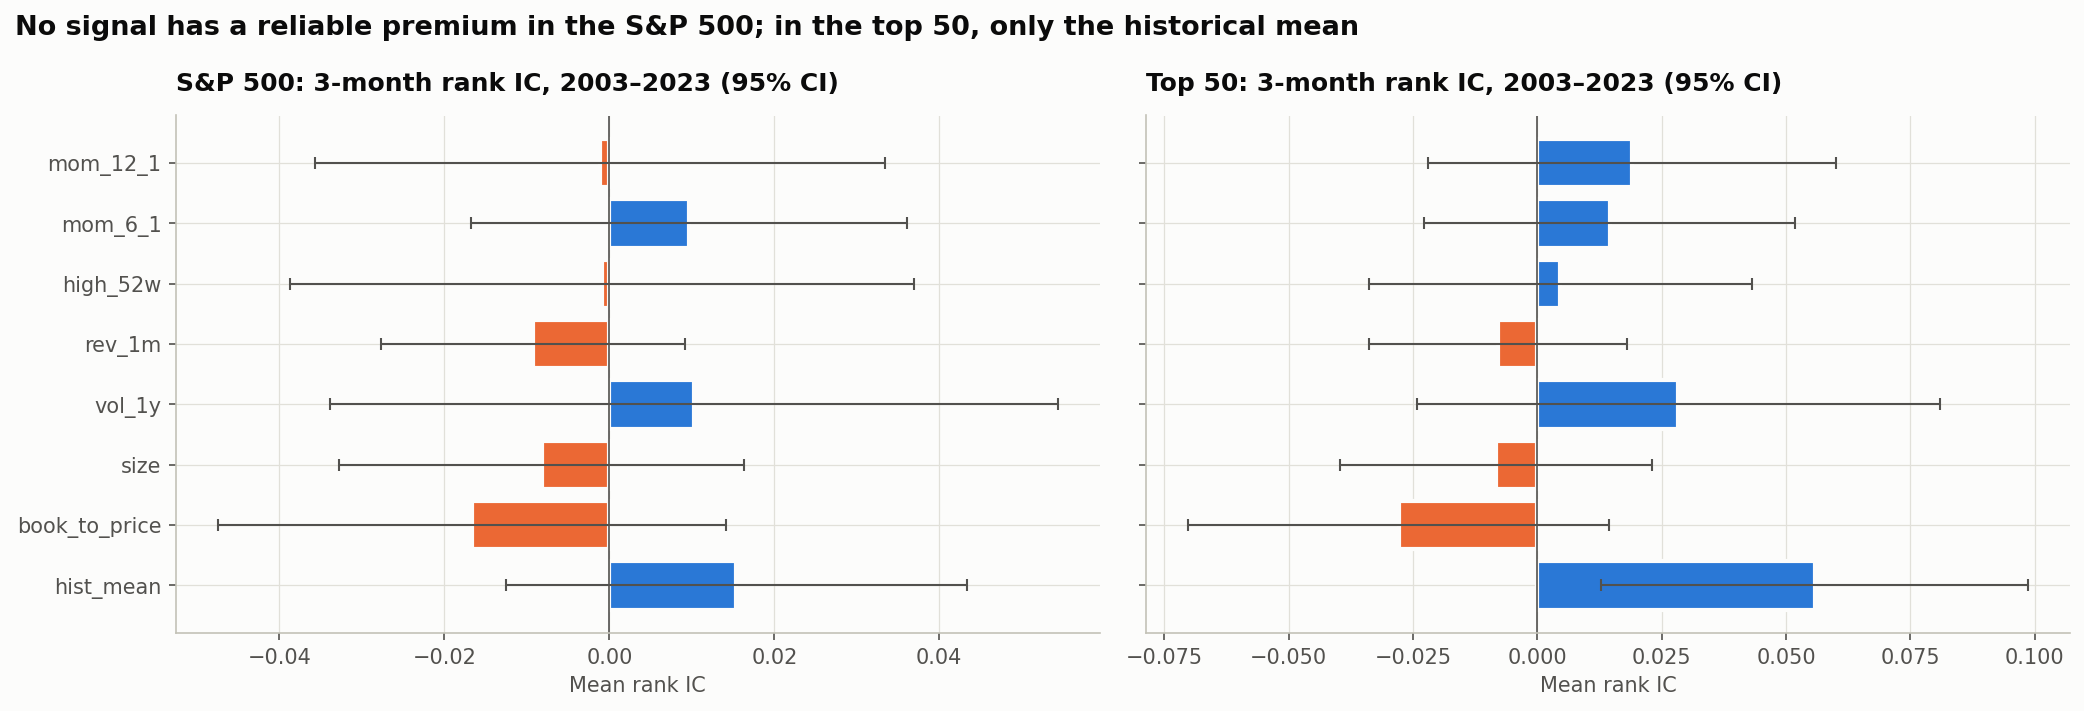
\includegraphics[width=0.84\textwidth]{phase5_ic.png}
\notecaption{\textbf{Figure 2.} Mean 3-month rank IC by signal, 2003--2023, with 95\% intervals.}\end{figure}

\section{Fixing the portfolio construction}
Signals were turned into expected returns with Grinold's rule, $\alpha_i = \text{IC}\times\omega_i\times z_i$, the IC
estimated only from past data and $\omega_i$ each stock's specific volatility from a statistical factor risk model
(five principal components). A benchmark-relative optimiser then maximises
$h\,\alpha^\top(w-b) - h\,\lambda\,(w-b)^\top\Sigma(w-b) - c\,\lVert w-w_{\text{current}}\rVert_1$ against the
cap-weighted top 50, with $\lambda = 10$ set from Grinold's rule for the optimal tracking error and trades charged
at their real cost.

\begin{table}[H]\centering\small
\notecaption{\textbf{Table 2.} Portfolio construction, 2010--2023, after costs (Sharpe ratios with the constant 3\%).}
\begin{tabular}{lrrr}\toprule
& Sharpe & Turnover / yr & Max drawdown\\\midrule
Baseline (momentum, ARIMA views, max-Sharpe) & 0.52 & 453\% & $-$33.0\% \\
Max-Sharpe with Grinold alpha, historical mean & 0.54 & 144\% & $-$50.5\% \\
Max-Sharpe with Grinold alpha, momentum & 0.42 & 344\% & $-$32.3\% \\
Benchmark-relative, historical mean & 0.54 & 28\% & $-$31.3\% \\
Benchmark-relative, momentum & 0.54 & 25\% & $-$29.5\% \\
Cap-weighted top 50 & 0.53 & 22\% & $-$30.0\% \\
\bottomrule\end{tabular}
\end{table}
\vspace{-0.3cm}
With the same alpha, max-Sharpe turns a historical-mean signal into 144\% turnover and a $-$50.5\% drawdown, and a
momentum alpha whose cross-sectional standard deviation is under 1\% a year into 344\% turnover. The
benchmark-relative optimiser holds 44--48 names, transfers the signal to the weights (transfer coefficient 0.72
for the historical mean), and earns +0.3\% a year over its benchmark at 1.6\% tracking error (IR 0.16, t = 0.61). The construction
problem is solved; what it reveals is that the alphas are worth very little.

Two standard momentum refinements were also tested. Volatility management (Barroso and Santa-Clara, 2015) transforms
the long-short momentum factor: maximum drawdown $-$71.8\% $\rightarrow$ $-$29.5\%, worst month $-$33.6\% $\rightarrow$
$-$11.3\%, Sharpe ratio $-$0.05 $\rightarrow$ 0.31 (t = 1.50). Residual momentum (Blitz et al., 2011) is steadier
than 12--1 momentum in the top 50 but has no premium in the S\&P 500. Neither helps the long-only top-50 portfolio.
The risk model's tracking-error forecasts were accurate for random portfolios (bias statistic 0.98) and specific
risk (0.98) but too low for optimised ones; adding the alpha as a risk factor (Lee and Stefek, 2008) brings the
historical-mean portfolio from 1.17 to 1.10.

\section{Attribution and multiple testing}\label{sec:inference}
All 47 variants were rebuilt over 2010--2023 and tested against the S\&P 500 proxy with the actual T-bill rate.
Attribution is relative to the proxy, because the price data lacks dividends while the Fama--French factors include
them. Sharpe-ratio differences are tested with a circular block bootstrap (21-day blocks, 2,000 resamples).

\begin{table}[H]\centering\small
\notecaption{\textbf{Table 3.} Inference, 2010--2023. Factor alpha and loadings: regression of returns relative to the
S\&P 500 proxy on the Fama--French five factors plus momentum, Newey--West t-statistics.}
\begin{tabular}{lrrrrrr}\toprule
& Sharpe & Difference & Bootstrap & Factor alpha & Momentum & Investment\\
& (T-bill) & vs S\&P 500 & p & a year (t) & loading & (CMA) loading\\\midrule
Baseline & 0.625 & $-$0.015 & 0.91 & +0.69\% (+0.30) & +0.22 & $-$0.24 \\
Best by Sharpe: max weight 10\% & 0.715 & +0.075 & 0.51 & +1.67\% (+0.97) & +0.20 & $-$0.16 \\
Best by IR: ARIMA views corrected & 0.703 & +0.063 & 0.66 & +2.41\% (+1.02) & +0.23 & $-$0.33 \\
Benchmark-relative, historical mean & 0.660 & +0.020 & 0.73 & +0.34\% (+0.43) & +0.04 & $-$0.14 \\
\bottomrule\end{tabular}
\end{table}
\vspace{-0.3cm}
\begin{itemize}\setlength\itemsep{1pt}
\item \textbf{Factor tilts, not alpha.} The baseline is long momentum (t = 10.5) and tilted against conservative-investment
and value stocks; across all 47 variants factor alpha t-statistics range from $-$1.79 to +1.02. No
Sharpe-ratio difference is significant (smallest p-value 0.37).
\item \textbf{Deflated Sharpe ratio} (Bailey and L\'opez de Prado, 2014). The best information ratio, 0.338, exceeds the
0.238 that luck alone would give from 47 independent tries; the deflated Sharpe ratio is 0.65, or 0.80--0.85
allowing for how correlated the variants are (2--4 effective trials).
\item \textbf{Overfitting} (Bailey et al., 2017). Within each group of variants against its own benchmark, the probability of
backtest overfitting is 0.49 and 0.65, and the in-sample winner's IR falls from about 0.5 to 0.12 and 0.01 out of sample.
\end{itemize}

\begin{figure}[H]\centering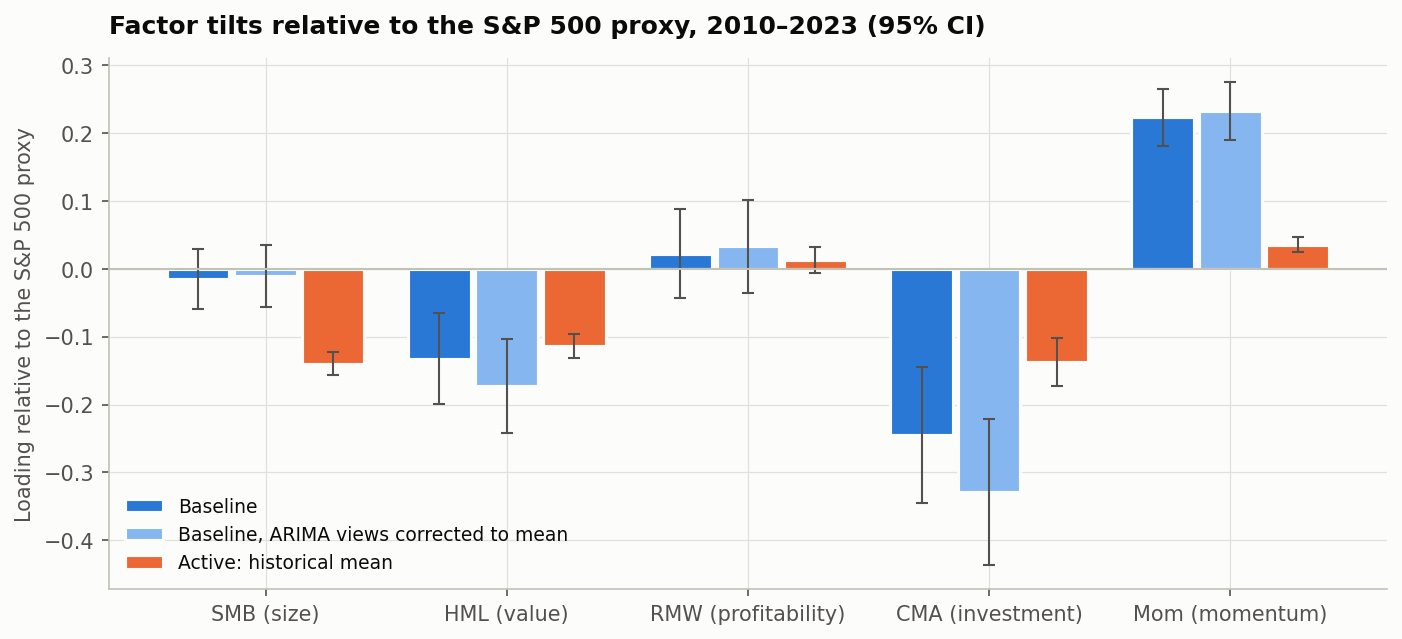
\includegraphics[width=0.58\textwidth]{phase8_factor_tilts.png}
\notecaption{\textbf{Figure 3.} Factor loadings relative to the S\&P 500 proxy, 2010--2023, with 95\% intervals.}\end{figure}

\begin{figure}[H]\centering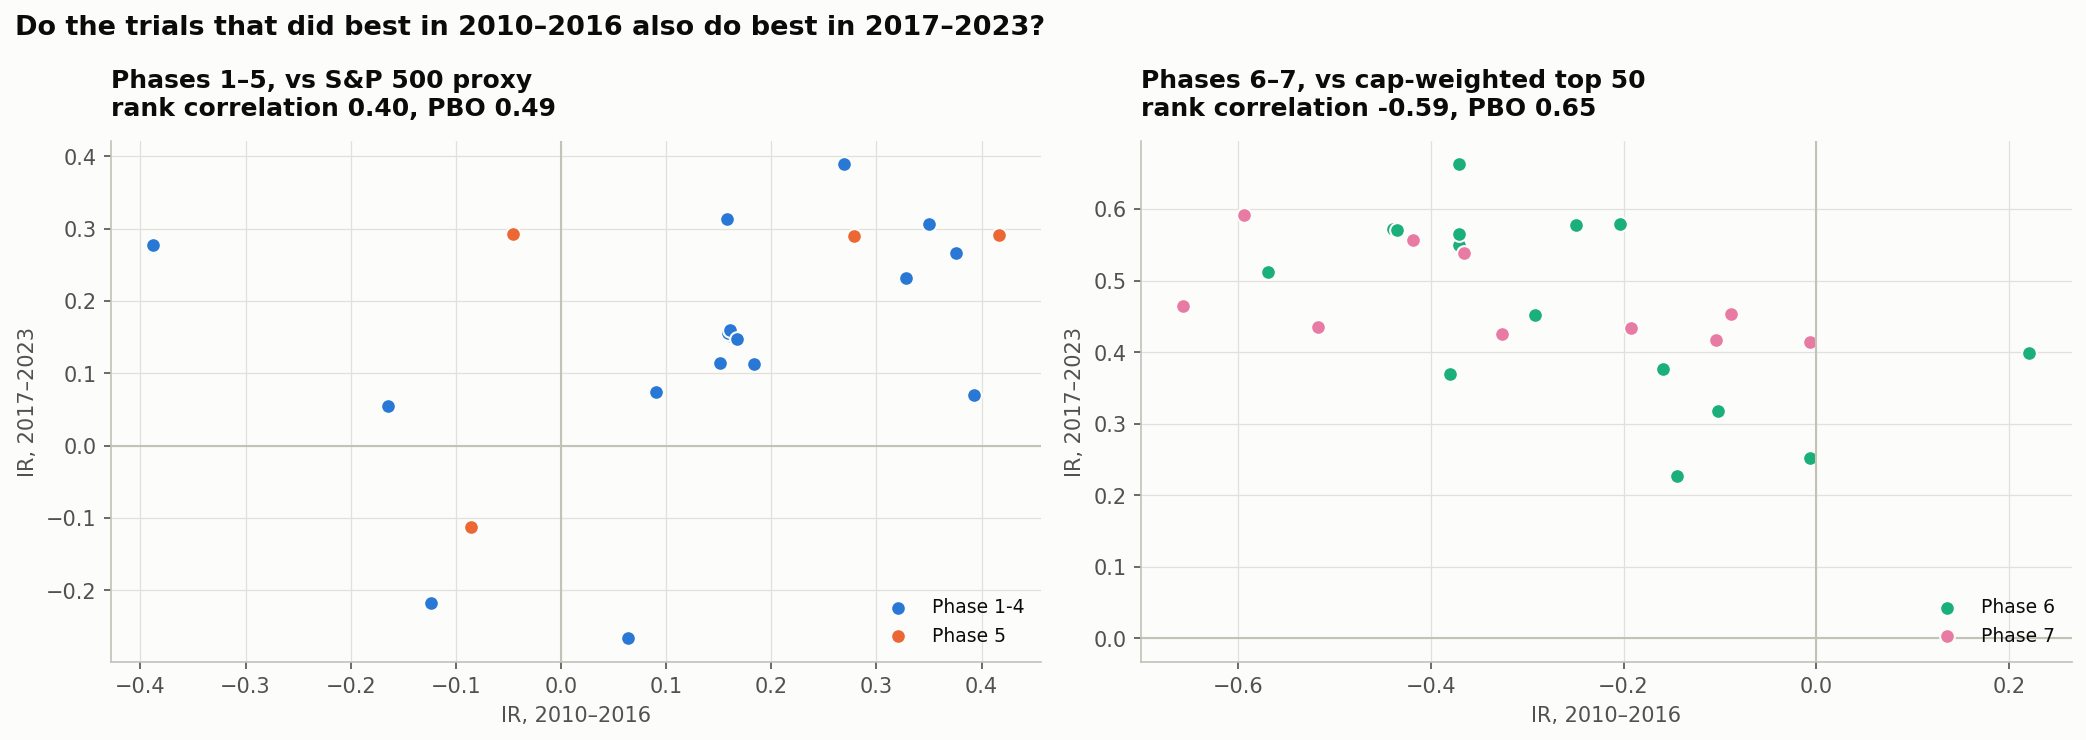
\includegraphics[width=0.84\textwidth]{phase8_overfitting.png}
\notecaption{\textbf{Figure 4.} Information ratios of each variant in 2010--2016 and 2017--2023, by group.}\end{figure}

\section{Conclusions}
Large-cap momentum offered no premium in 2003--2023, and the strategy's apparent edge over the S\&P 500 is a
momentum-and-growth tilt that disappears under factor attribution, the actual risk-free rate and corrections for
the number of variants tried. The more durable lessons are methodological: a max-Sharpe optimiser converts weak
forecasts into concentrated, high-turnover bets; a benchmark-relative optimiser with risk and cost penalties
expresses the same forecasts as small, cheap tilts; risk forecasts for optimised portfolios fail when the risk model
does not contain the alpha; and the best of many backtests is weak evidence until deflated.

\textbf{Limitations.} Price returns only (no dividends); no sector data; linear transaction costs; one market and
period (2003--2023); the 47 variants are a lower bound on what was tried. The natural next test is out-of-sample data
from 2024 onwards, with the settings fixed now.

\section*{References}
\footnotesize
\begin{description}\setlength\itemsep{0pt}
\item Bailey, D. H. and L\'opez de Prado, M. (2014). The deflated Sharpe ratio. \emph{Journal of Portfolio Management} 40(5).
\item Bailey, D. H., Borwein, J., L\'opez de Prado, M. and Zhu, Q. J. (2017). The probability of backtest overfitting. \emph{Journal of Computational Finance} 20(4).
\item Barroso, P. and Santa-Clara, P. (2015). Momentum has its moments. \emph{Journal of Financial Economics} 116(1).
\item Black, F. and Litterman, R. (1992). Global portfolio optimization. \emph{Financial Analysts Journal} 48(5).
\item Blitz, D., Huij, J. and Martens, M. (2011). Residual momentum. \emph{Journal of Empirical Finance} 18(3).
\item Clarke, R., de Silva, H. and Thorley, S. (2002). Portfolio constraints and the fundamental law of active management. \emph{Financial Analysts Journal} 58(5).
\item Fama, E. F. and French, K. R. (2015). A five-factor asset pricing model. \emph{Journal of Financial Economics} 116(1).
\item Fama, E. F. and MacBeth, J. D. (1973). Risk, return, and equilibrium. \emph{Journal of Political Economy} 81(3).
\item Grinold, R. C. and Kahn, R. N. (2000). \emph{Active Portfolio Management}, 2nd ed. McGraw-Hill.
\item He, G. and Litterman, R. (1999). The intuition behind Black--Litterman model portfolios. Goldman Sachs.
\item Jegadeesh, N. and Titman, S. (1993). Returns to buying winners and selling losers. \emph{Journal of Finance} 48(1).
\item Ledoit, O. and Wolf, M. (2004). A well-conditioned estimator for large-dimensional covariance matrices. \emph{Journal of Multivariate Analysis} 88(2).
\item Lee, J.-H. and Stefek, D. (2008). Do risk factors eat alphas? \emph{Journal of Portfolio Management} 34(4).
\item Newey, W. K. and West, K. D. (1987). A simple, positive semi-definite, heteroskedasticity and autocorrelation consistent covariance matrix. \emph{Econometrica} 55(3).
\end{description}
\end{document}
